\documentclass[tikz,border=4pt]{standalone}
\usepackage{amsmath}
\begin{document}
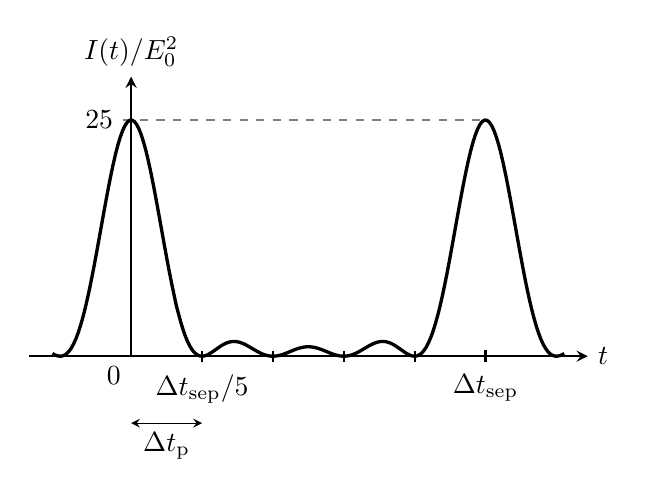
\begin{tikzpicture}[>=stealth, thick, scale=1.0]
  % Axes: horizontal u = t / Delta t_sep from -0.25 to 1.25, scaled by 4.5
  % vertical: I(t)/E_0^2 from 0 to 25, scaled by 0.12 (so 25 -> 3.0)
  \draw[->] (-1.3, 0) -- (5.8, 0) node[right] {$t$};
  \draw[->] (0, 0) -- (0, 3.55) node[above] {$I(t)/E_0^2$};
  \node[below left] at (0, 0) {$0$};

  % Peak height label 25
  \draw[dashed, thin, black!50] (-0.1, 3.0) -- (4.5, 3.0);
  \node[left] at (-0.1, 3.0) {$25$};

  % Plot (sin(5*pi*u)/sin(pi*u))^2 * 0.12 where u = \x / 4.5
  \draw[very thick, domain=-1.0:5.5, samples=220]
    plot (\x, {0.12 * pow(1 + 2*cos(deg(2*pi*\x/4.5)) + 2*cos(deg(4*pi*\x/4.5)), 2)});

  % Ticks for zeros and Delta t_sep
  \foreach \k in {1, 2, 3, 4} {
    \draw (\k*0.9, 0.07) -- (\k*0.9, -0.07);
  }
  \draw (4.5, 0.08) -- (4.5, -0.08);
  \node[below] at (0.9, -0.1) {$\Delta t_{\mathrm{sep}}/5$};
  \node[below] at (4.5, -0.1) {$\Delta t_{\mathrm{sep}}$};

  % Indicate pulse width Delta t_p cleanly below
  \draw[<->, thin] (0, -0.85) -- (0.9, -0.85) node[midway, below] {$\Delta t_{\mathrm{p}}$};
\end{tikzpicture}
\end{document}
